
\begin{question}
Please make a frequency histogram from the following (unsorted)
continuous data by rounding to the nearest integer.

\begin{longtable}[]{@{}rrrrrr@{}}
\toprule
41.3569 & 42.1693 & 42.3342 & 42.4591 & 47.0093 & 42.1409\tabularnewline
42.2758 & 40.8129 & 43.2877 & 45.6308 & 41.6567 & 40.9801\tabularnewline
41.8061 & 41.2497 & 47.1675 & 47.5627 & 46.0522 & 42.1835\tabularnewline
43.9473 & 41.7718 & 41.0139 & 42.4773 & 43.6446 & 41.0095\tabularnewline
\bottomrule
\end{longtable}
\end{question}

\begin{solution}
Make a frequency table.

\begin{longtable}[]{@{}rr@{}}
\toprule
value & frequency\tabularnewline
\midrule
\endhead
41 & 6\tabularnewline
42 & 10\tabularnewline
43 & 1\tabularnewline
44 & 2\tabularnewline
45 & 0\tabularnewline
46 & 2\tabularnewline
47 & 2\tabularnewline
48 & 1\tabularnewline
\bottomrule
\end{longtable}

Make the histogram.

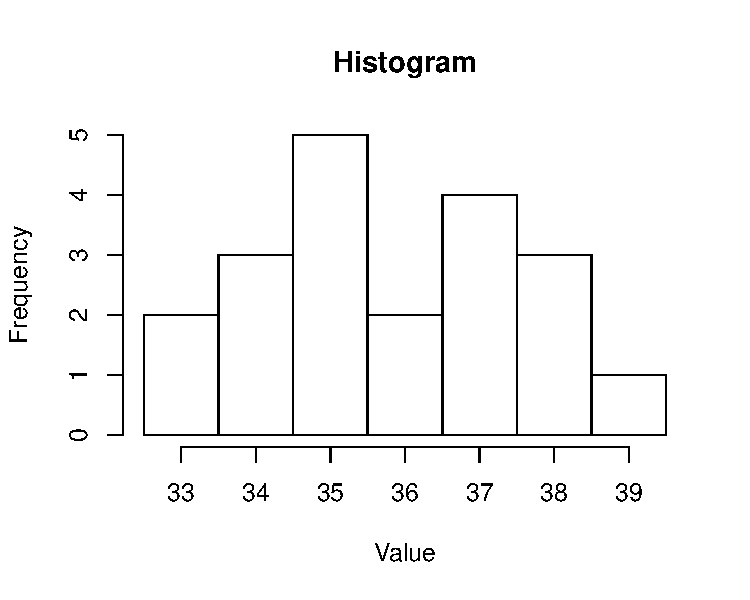
\includegraphics{barchart-1.pdf}\\
\end{solution}

